\documentclass[a4paper,12pt]{article} 

\usepackage[unicode, pdftex]{hyperref}

%Добавляет возможность искать и копировать текст
\usepackage{cmap}

%Убирает пробел между названием таблицы/рисунка и самой таблицей/рисунком
\usepackage{caption}
\captionsetup[table]{skip= -0 cm}
\captionsetup[figure]{skip= -0 cm}

%Выравнивание названия таблиц по левому краю
%\usepackage[nooneline]{caption} 
%Размеры отступов 
\usepackage[left=20mm, top=20mm, right=20mm, bottom=20mm, footskip=10mm]{geometry}

%Рисунки
\usepackage{graphicx}
\usepackage{wrapfig} %обтекание элементов
\graphicspath{{graphs}{figures}}  % папки с картинками

%Русский язык в формулах
\usepackage{mathtext}

%  Русский язык
\usepackage[T2A]{fontenc}			
\usepackage[utf8]{inputenc}			
\usepackage[english,russian]{babel}	

%Красная строка для первого абзаца
\usepackage{indentfirst}

%Готические буквы
\usepackage{amssymb}

% Математика
\usepackage{amsmath,amsfonts,amssymb,amsthm,mathtools} 
\usepackage{wasysym}

%Цветные подписи в таблице
\usepackage[table,xcdraw]{xcolor}

\usepackage{fancyhdr} % Колонтитулы
 	\pagestyle{fancy}
 	\renewcommand{\headrulewidth}{0.3mm}  % Толщина линейки, отчеркивающей верхний колонтитул
 	%\lfoot{Нижний левый}
 	%\rfoot{Нижний правый}
 	\rhead{Белостоцкий Артмемий, Б04-006}
 	%\chead{Верхний в центре}
 	\lhead{Лабораторная работа №5.5.1}
 	\renewcommand{\footrulewidth}{0.3mm}
 	\cfoot{\thepage} % По умолчанию здесь номер страницы
 	
 	
%\captionsetup[table]{
%  position=above,
%  justification=raggedright,
  %labelsep=newline, % <<< label and text on different lines
%  singlelinecheck=false % <<< raggadright also when the cap%tion is shorter
                        % than a single line
%}
 	
\begin{document} 

%Титульник 
\begin{titlepage}
	\begin{center}
		\large 	МИНИСТЕРСТВО ОБРАЗОВАНИЯ И НАУКИ РОССИЙСКОЙ ФЕДЕРАЦИИ\\
				МОСКОВСКИЙ ФИЗИКО-ТЕХНИЧЕСКИЙ ИНСТИТУТ \\
				(НАЦИОНАЛЬНЫЙ ИССЛЕДОВАТЕЛЬСКИЙ ИНСТИТУТ)\\ 
				ФИЗТЕХ-ШКОЛА ЭЛЕКТРОНИКИ, ФОТОНИКИ \\
				И МОЛЕКУЛЯРНОЙ ФИЗИКИ \\
		
		
		\vspace{4.0 cm}
		Лабораторная работа № 5.5.1 \\ 
		\LARGE \textbf{Измерение коэффициента ослабления потока $\gamma$-лучей в веществе и определение их энергии. Дозиметрия}
	\end{center}
	\vspace{3 cm} \large
	
	\begin{flushright}
		выполнил студент 3 курса \\
		{группы Б04-006}\\
		\textbf{Белостоцкий Артемий}\\
	\end{flushright}
	
	\vfill

	\begin{center}
	Долгопрудный, 2022 г.
	\end{center}
\end{titlepage}                                                                      

\section*{Аннотация}

В данной работе изучается затухание гамма-лучей в веществе -- свинце, железе и алюминии. Также измеряются коэффициенты ослабления потока гамма-лучей и по их величины определяется энергия гамма-квантов. Сверх того, будут получены практические навыки работы с дозиметром. 

\section*{Теоретические сведения}

Гамма-лучи возникают при переходе возбужденных ядер из одного энергетического состояния в другое, более низкое. Энергия $\gamma$-квантов обычно заключена между несколькими десятками кэВ и несколькими МэВ. Проходя через вещество, пучок $\gamma$-квантов постепенно ослабляется. Ослабление происходит по экспоненциальному закону который нетрудно вывести из физических соображений.

Считая, что при прохождении через вещество меняется лишь количество $\gamma$-квантов, но не их энергия, обозначим $-dN$ число $\gamma$-квантов, выбывших из пучка на пути $dl$. Это число пропорционально имеющимся их числу N и пройденному пути $dl$. Имеем, следовательно

\begin{align}
	-dN = \mu N dl \nonumber \\
	N = N_0 e^{-\mu l} \nonumber \\
	\mu = \frac{1}{l} \ln \left( \frac{N_0}{N} \right) \label{eq1}
\end{align}


\section*{Экспериментальная установка}

\begin{figure}[h]
	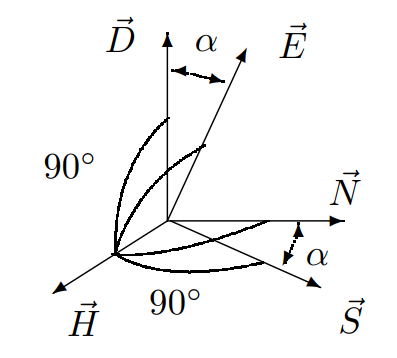
\includegraphics[width=\linewidth]{fig1}
	\caption{Экспериментальная установка. (1) -- свинцовый контейнер с коллиматорным каналом (после него стоит свинцовая пробка), (2) -- Сцинтилляционный счетчик}
	 \label{fig:setup1}
\end{figure}


\pagebreak

\begin{figure}[h]
	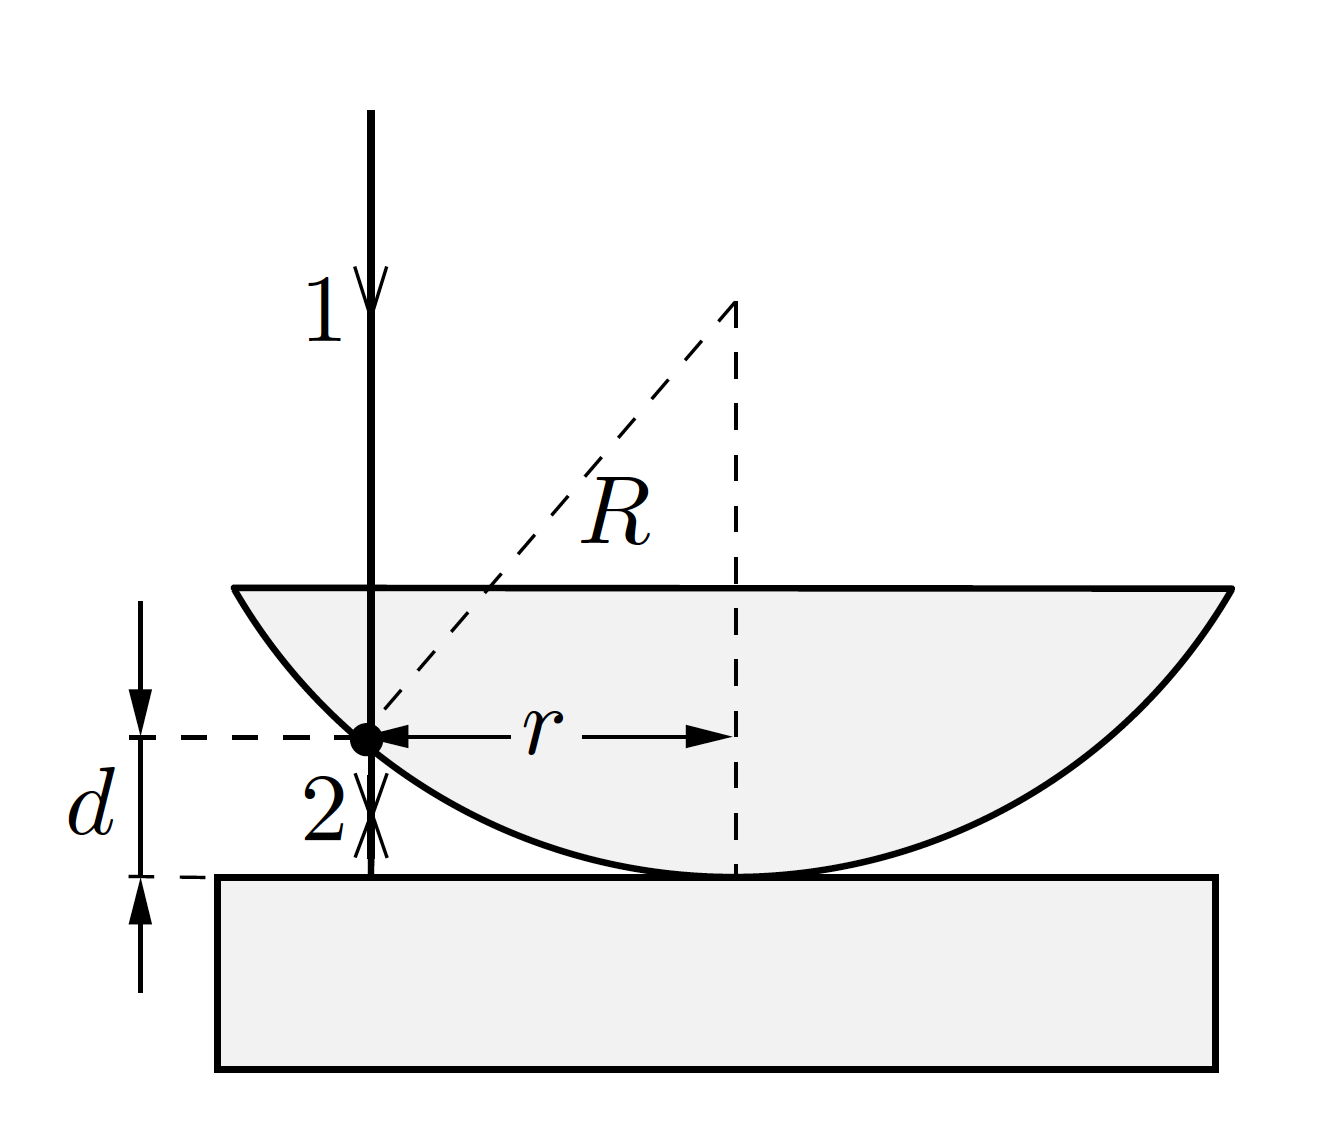
\includegraphics[width=\linewidth]{fig2}
	\caption{Электронная часть установки. (1) -- блок управления ФЭУ (состоит из вольтметра, ручек регулировки напряжения на ФЭУ (<<грубо>>, <<точно>>) и кнопки включения/выключения (<<Вкл>>) ) }
	\label{fig:setup2}
\end{figure}

\section*{Ход работы}

Методика измерений заключается в фиксировании времени, за которое счетчик зарегистрирует $10^5$ частиц в отсутствие ($N'_0$) и в присутствие (N') поглотителя в зависимости от толщины поглощающего слоя.

Для изменения толщины поглощающего слоя будем ставить на пути распространения излучения поглощающие пластинки из определенного материала. Суммарная толщина поглощающего слоя (l) есть сумма размеров каждой пластинки. Таким образом, погрешность измерения l на n-том шаге составляет $\sigma_l = \sqrt{n} * \sigma_{шт}$, где $\sigma_{шт}$ = 0.01 мм -- систематическая погрешность штангенциркуля

Предполагая, что регистрация каждой частицы не зависит от регистрации другой, а количество всех зарегистрированных частиц есть сумма данных независимых величин, выполнен <<закон $\sqrt{N}$>>. Таким образом погрешность измерений величины N' равна $\sigma_N' = \\ =\sqrt{N'}$. Тогда погрешность определения потока частиц (N) есть $\sigma_N = \frac{\sqrt{N'}}{t}$, где t -- время измерений.

Рассчитаем погрешность для величины $y = \ln \left( \frac{N_0}{N} \right)$:
\[
	\sigma_y = \sqrt{ \frac{1}{N_0 t_0^2} + \frac{1}{N t^2}},
\]

где $t_0$ -- время измерения $N_0'$, $t$ -- время измерения $N'$. В данной работе $N, N_0 \sim 10^5$, тогда $\frac{\sigma_y}{y} \ll 1$

Включим установку и, перекрыв коллиматорный канал свинцовой пробкой измерим фон, который обусловлен шумом ФЭУ и посторонними частицами, получим: $N_{фон} = \\= (40,6 \pm 2,0) \ c^{-1}$. Далее будет видно, что $N_0, N \gg N_{фон}$, тогда формула \ref{eq1} не изменит свой вид.



\subsubsection*{Измерения для свинца}

По полученным данным, представленным в Таблице \ref{table1} построим зависимость $\ln(N_0/N) = \\ =\mu l$

\begin{figure}[h]
	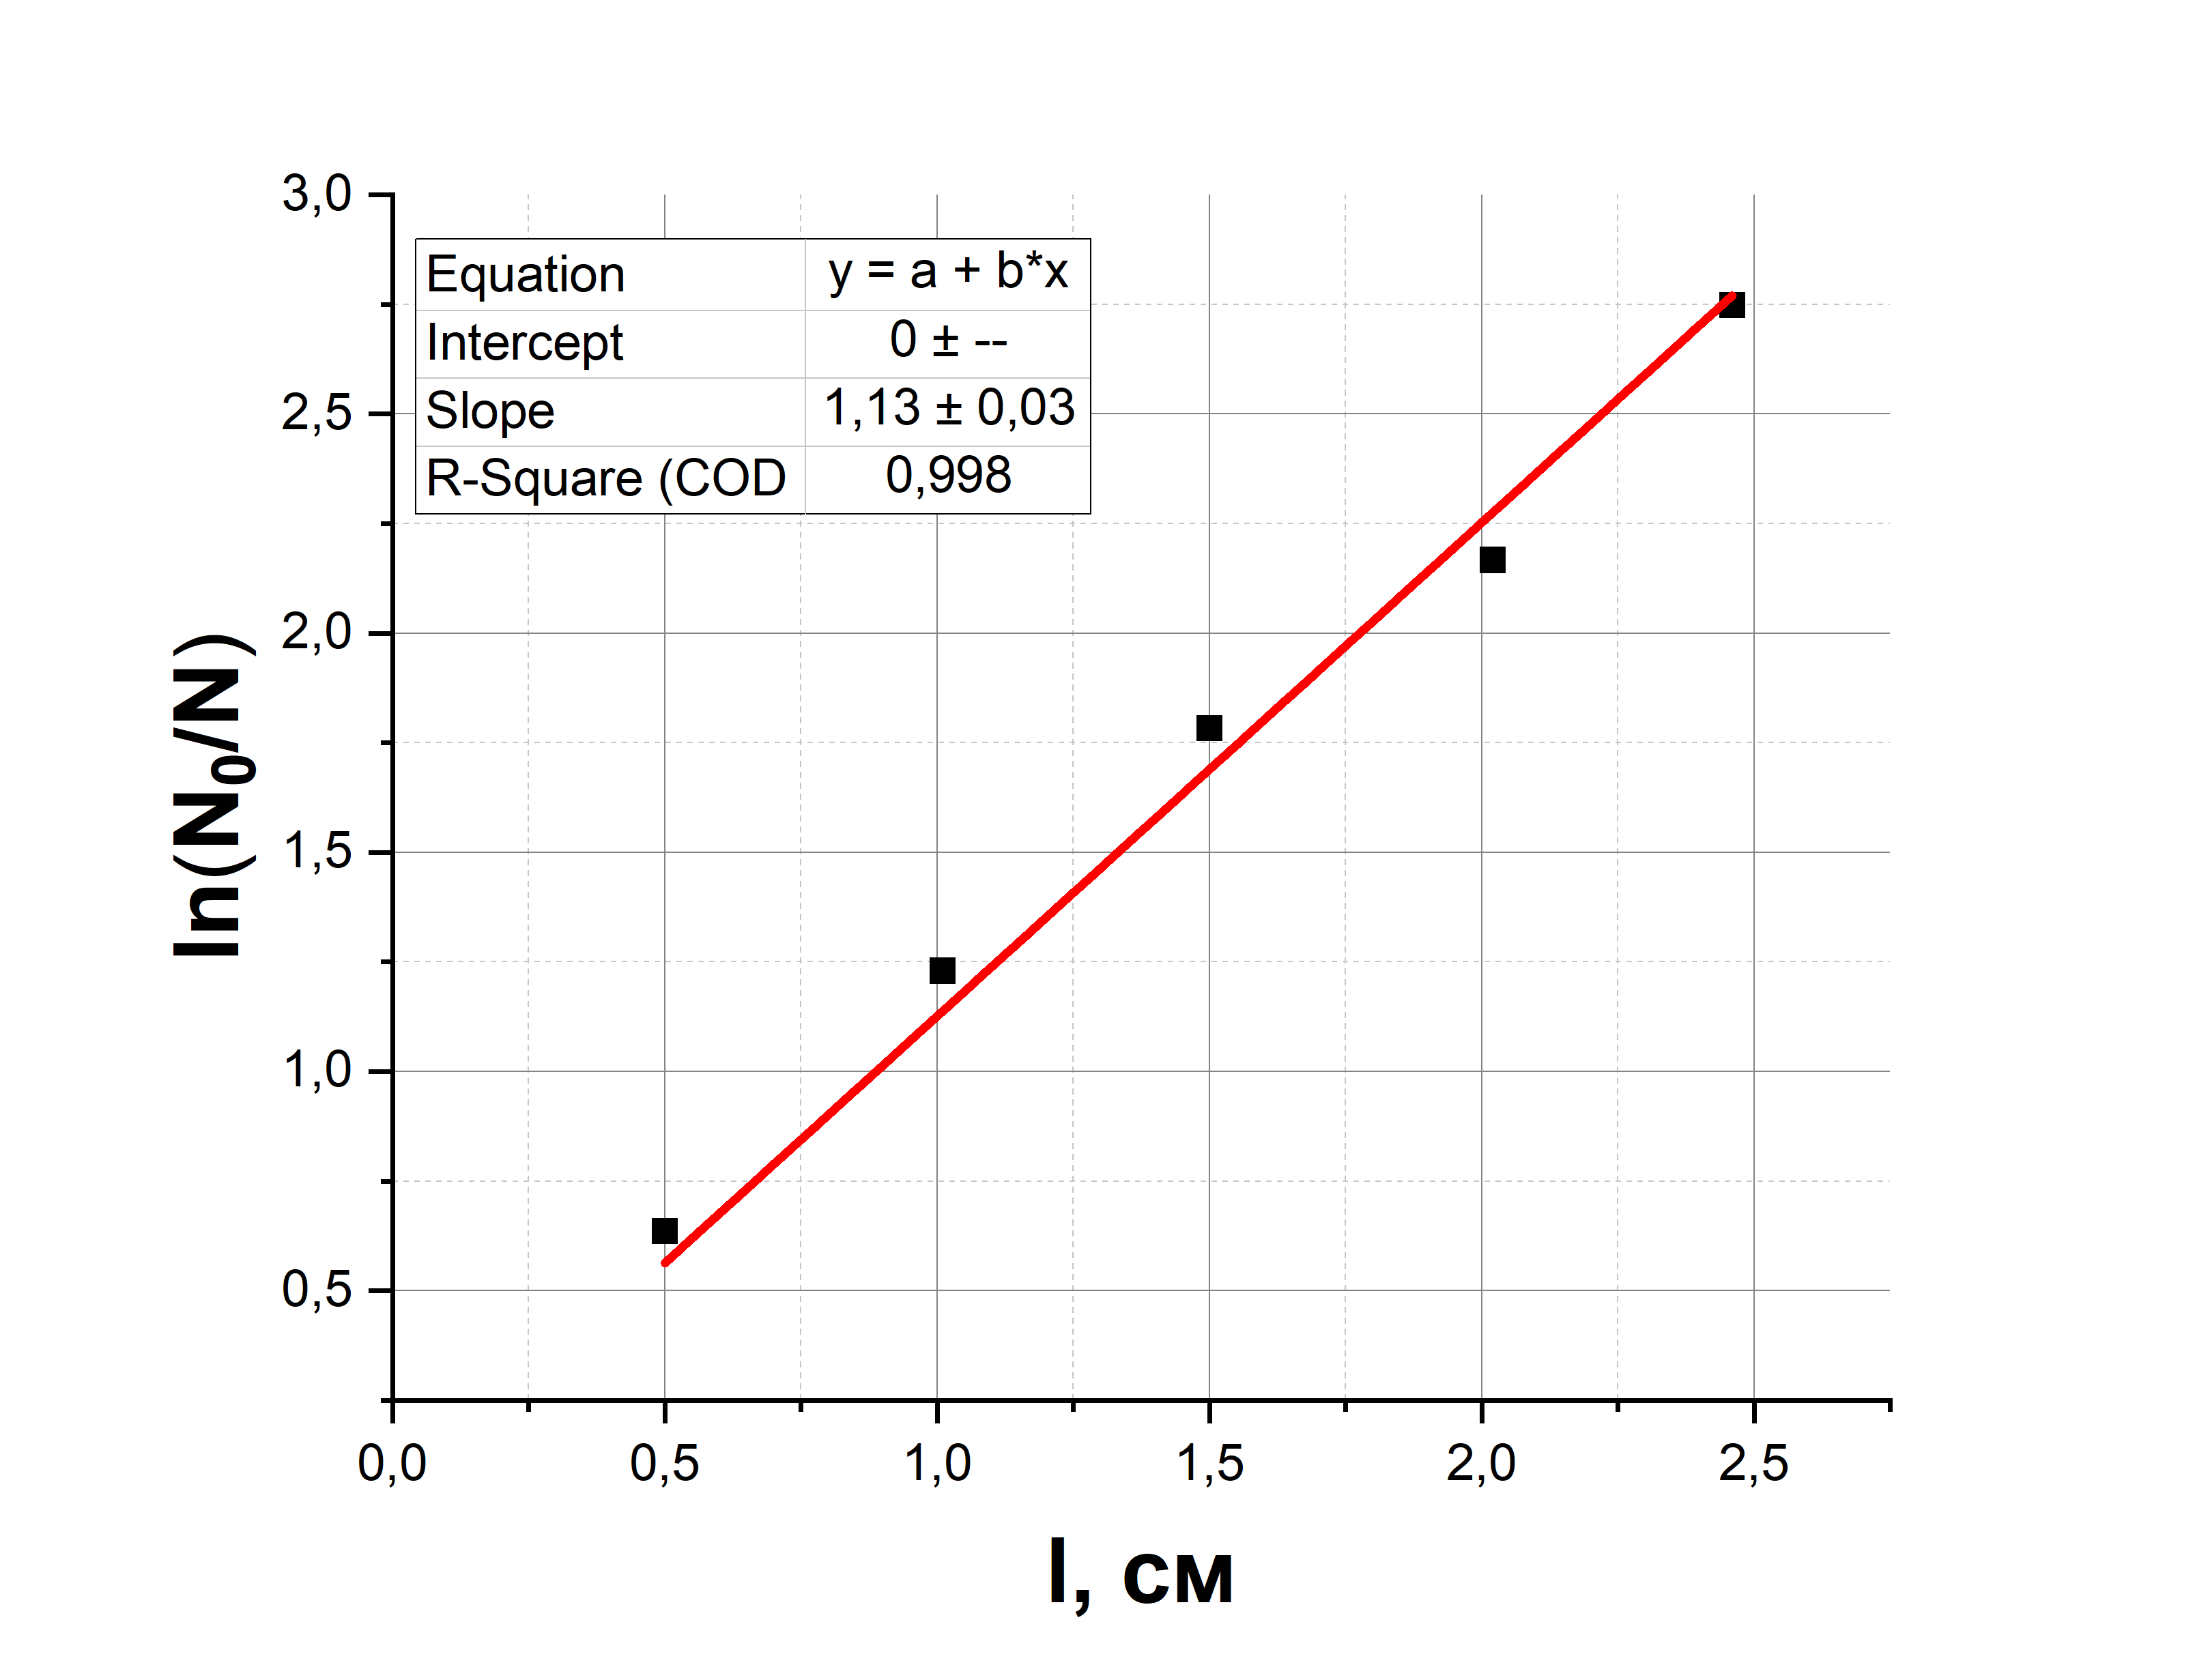
\includegraphics[width=\linewidth]{graph1(Pb)} 
	\caption{Зависимость логарифма отношений потоков частиц от толщины образца свинца.}
	\label{Pb}
\end{figure}

Получим, что для свинца линейный коэффициент поглощения $\gamma$-лучей -- \\ $\mu = (1,13 \pm 0,03) см^{-1}$. Данный коэффициент соответствует $\gamma$-квантам с энергией $E_{\gamma}$ = \\ = 0,6 -- 0,8 МэВ 



\newpage

\subsubsection*{Измерения для алюминия}

По полученным данным, представленным в Таблице \ref{table2} построим зависимость $\ln(N_0/N) = \\ =\mu l$

\begin{figure}[h]
	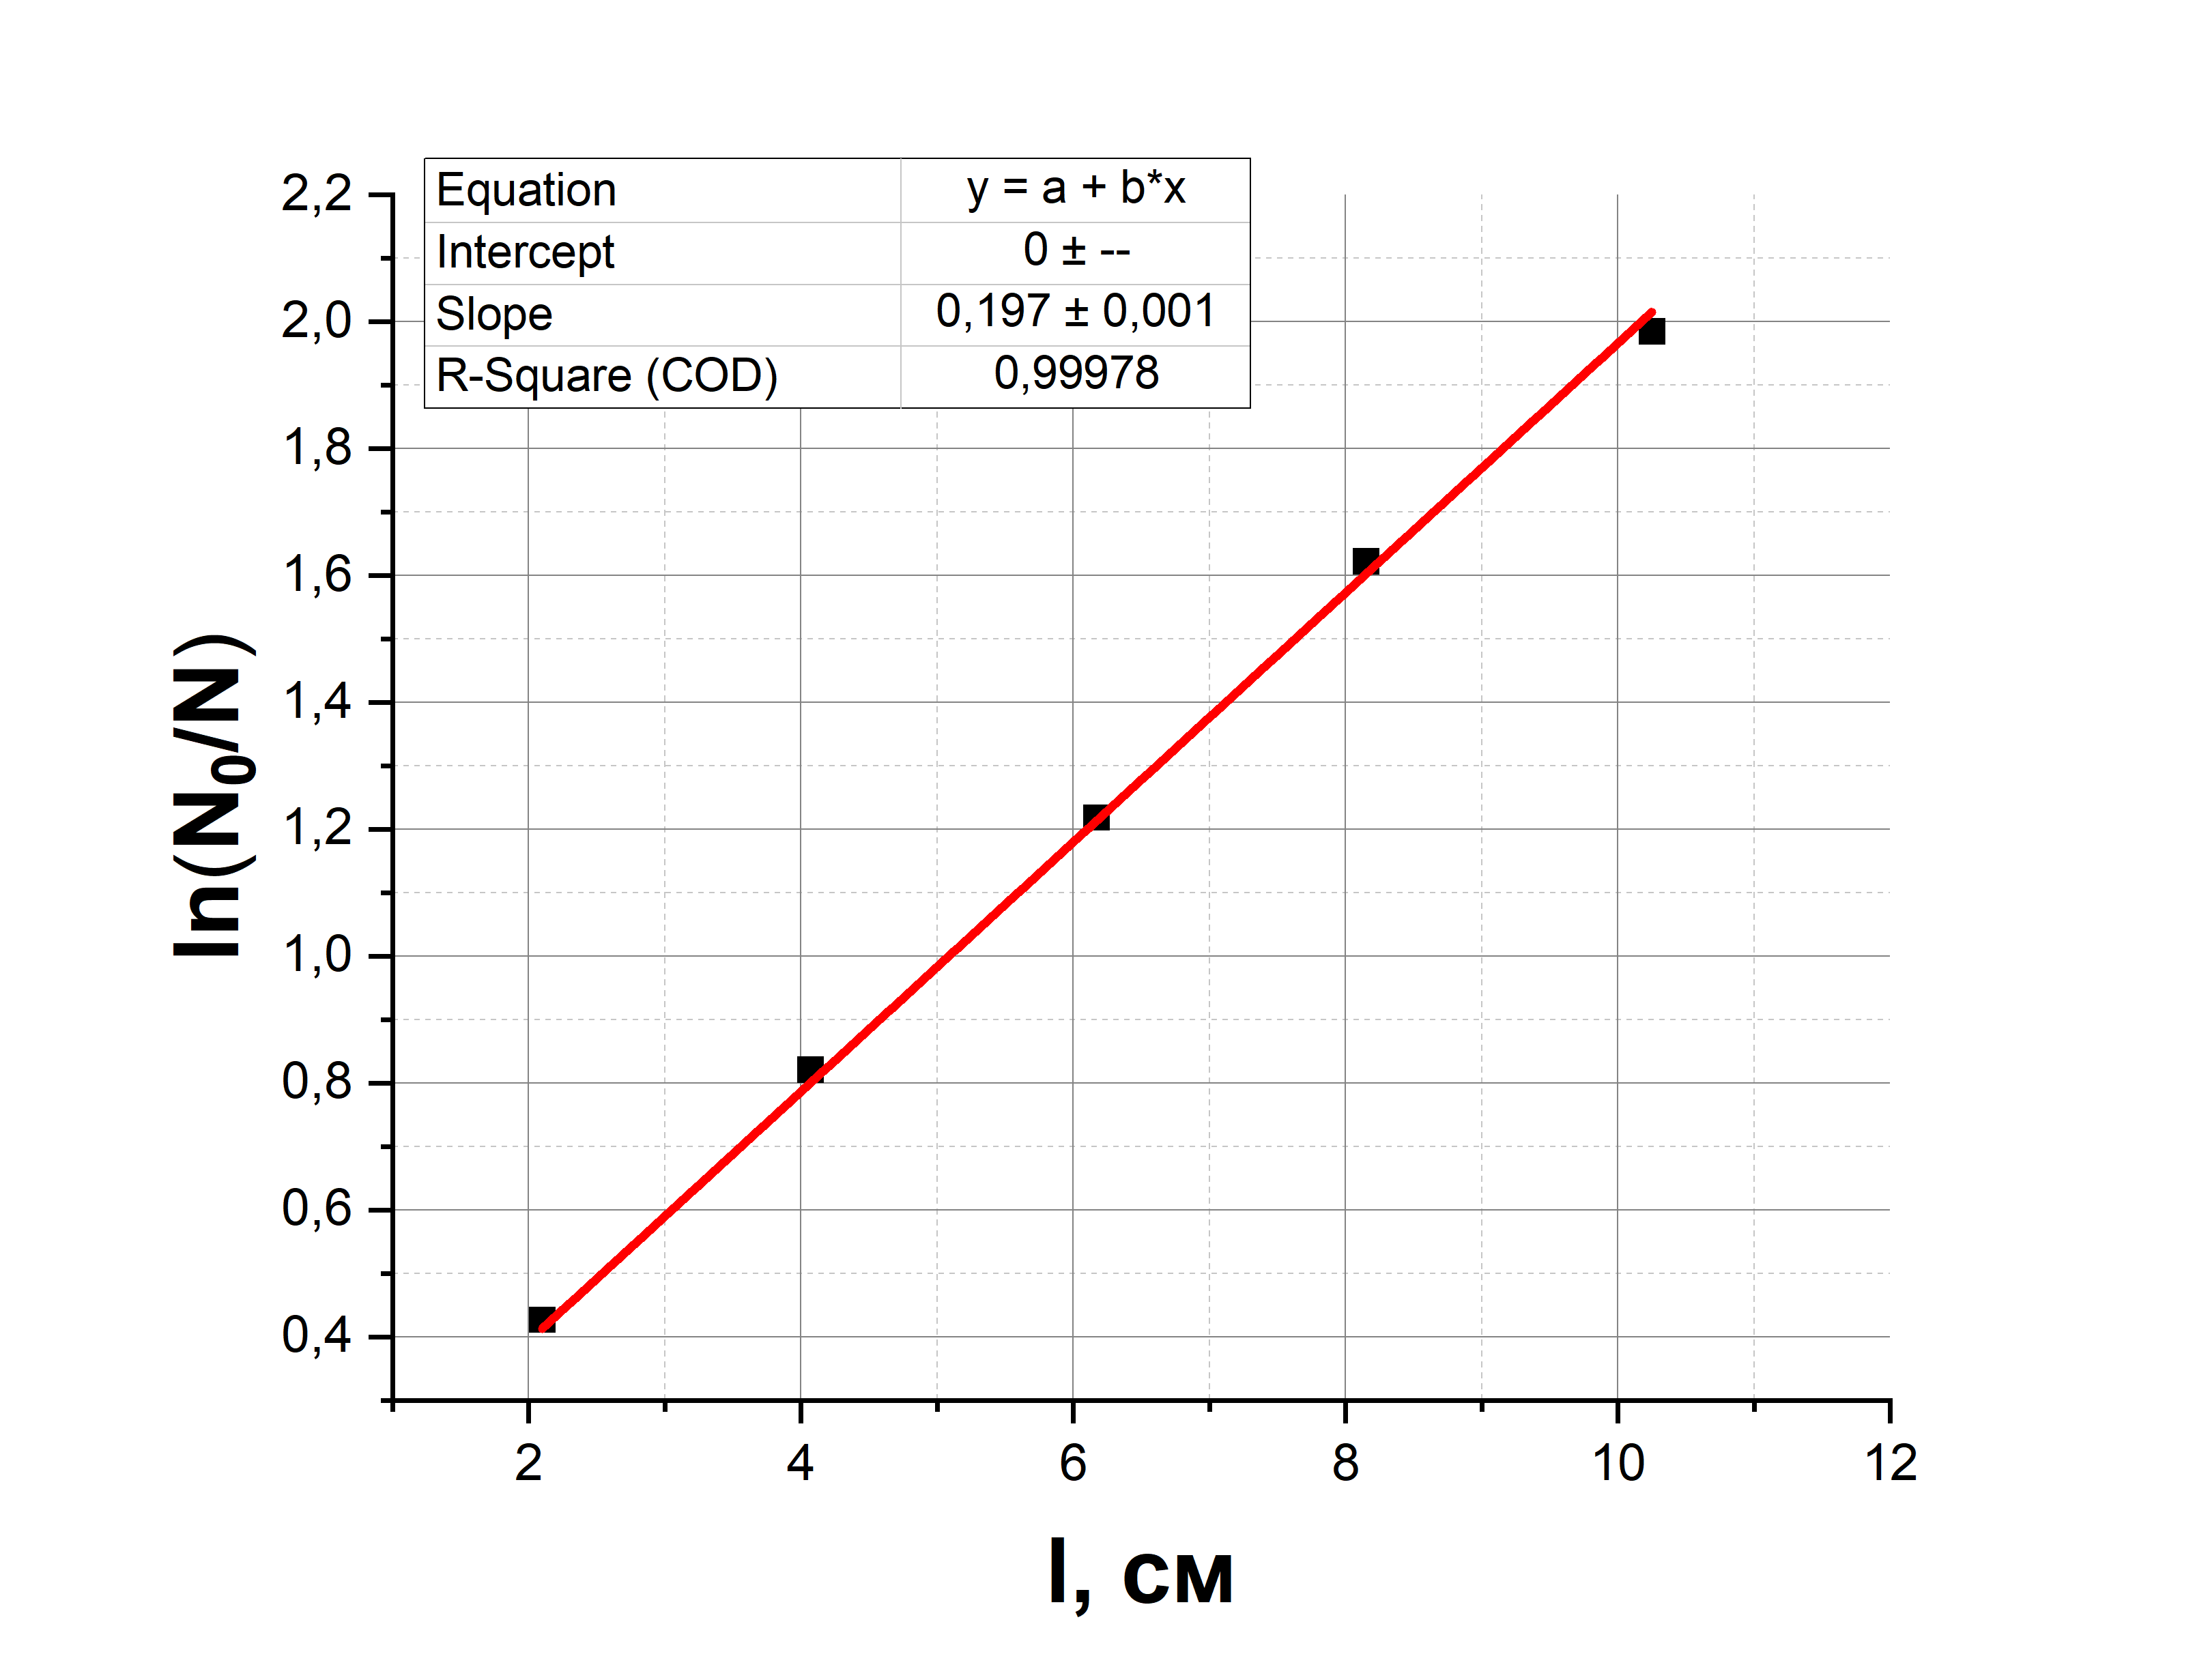
\includegraphics[width=\linewidth]{graph2(Al)} 
	\caption{Зависимость логарифма отношений потоков частиц от толщины образца алюминия.}
	\label{Al}
\end{figure}

Получим, что для свинца линейный коэффициент поглощения $\gamma$-лучей -- \\ $\mu = (0,197 \pm 0,001) см^{-1}$. Данный коэффициент соответствует $\gamma$-квантам с энергией $E_{\gamma}$ = \\ = 0,6 -- 0,8 МэВ 

\newpage

\subsubsection*{Измерения для железа}

По полученным данным, представленным в Таблице \ref{table3} построим зависимость $\ln(N_0/N) = \\ =\mu l$

\begin{figure}[h]
	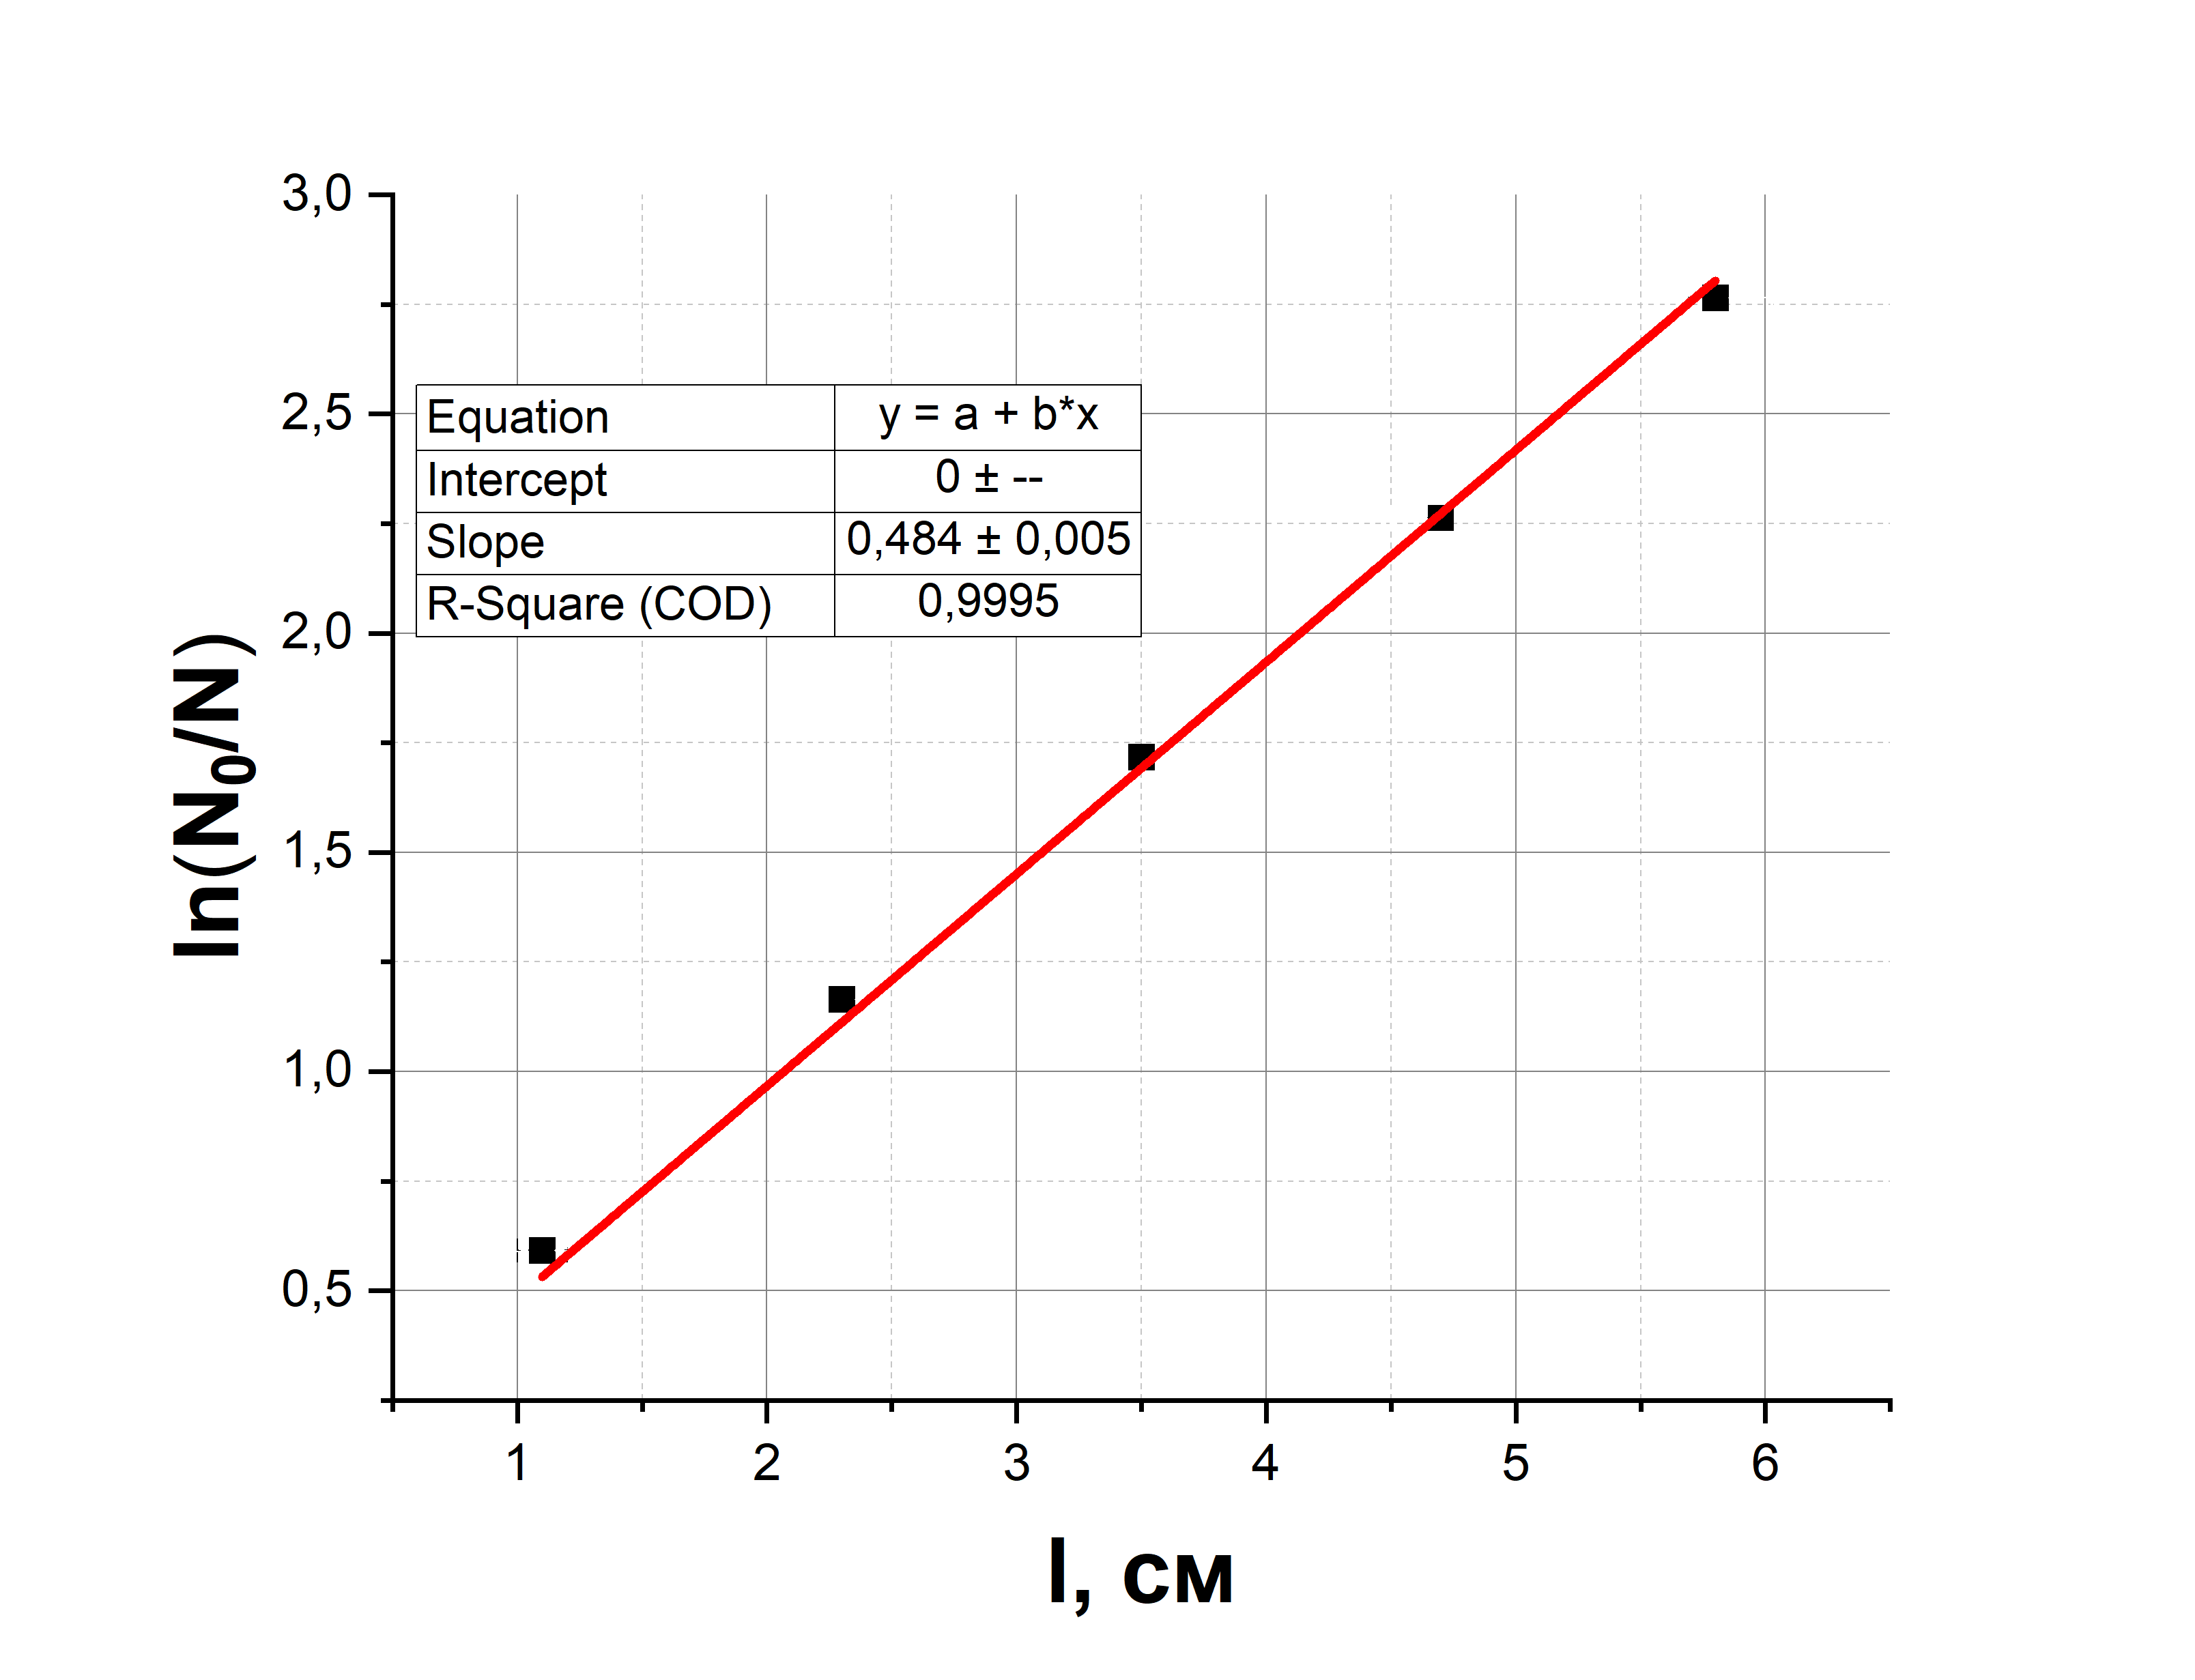
\includegraphics[width=\linewidth]{graph3(Fe)} 
	\caption{Зависимость логарифма отношений потоков частиц от толщины образца железа.}
	\label{Fe}
\end{figure}

Получим, что для свинца линейный коэффициент поглощения $\gamma$-лучей -- \\ $\mu = (0,484 \pm 0,005) см^{-1}$. Данный коэффициент соответствует $\gamma$-квантам с энергией $E_{\gamma}$ = \\ = 0,8 -- 1,0 МэВ 

\newpage

\section*{Дозиметрия}

\begin{figure}[h]
	\centering
	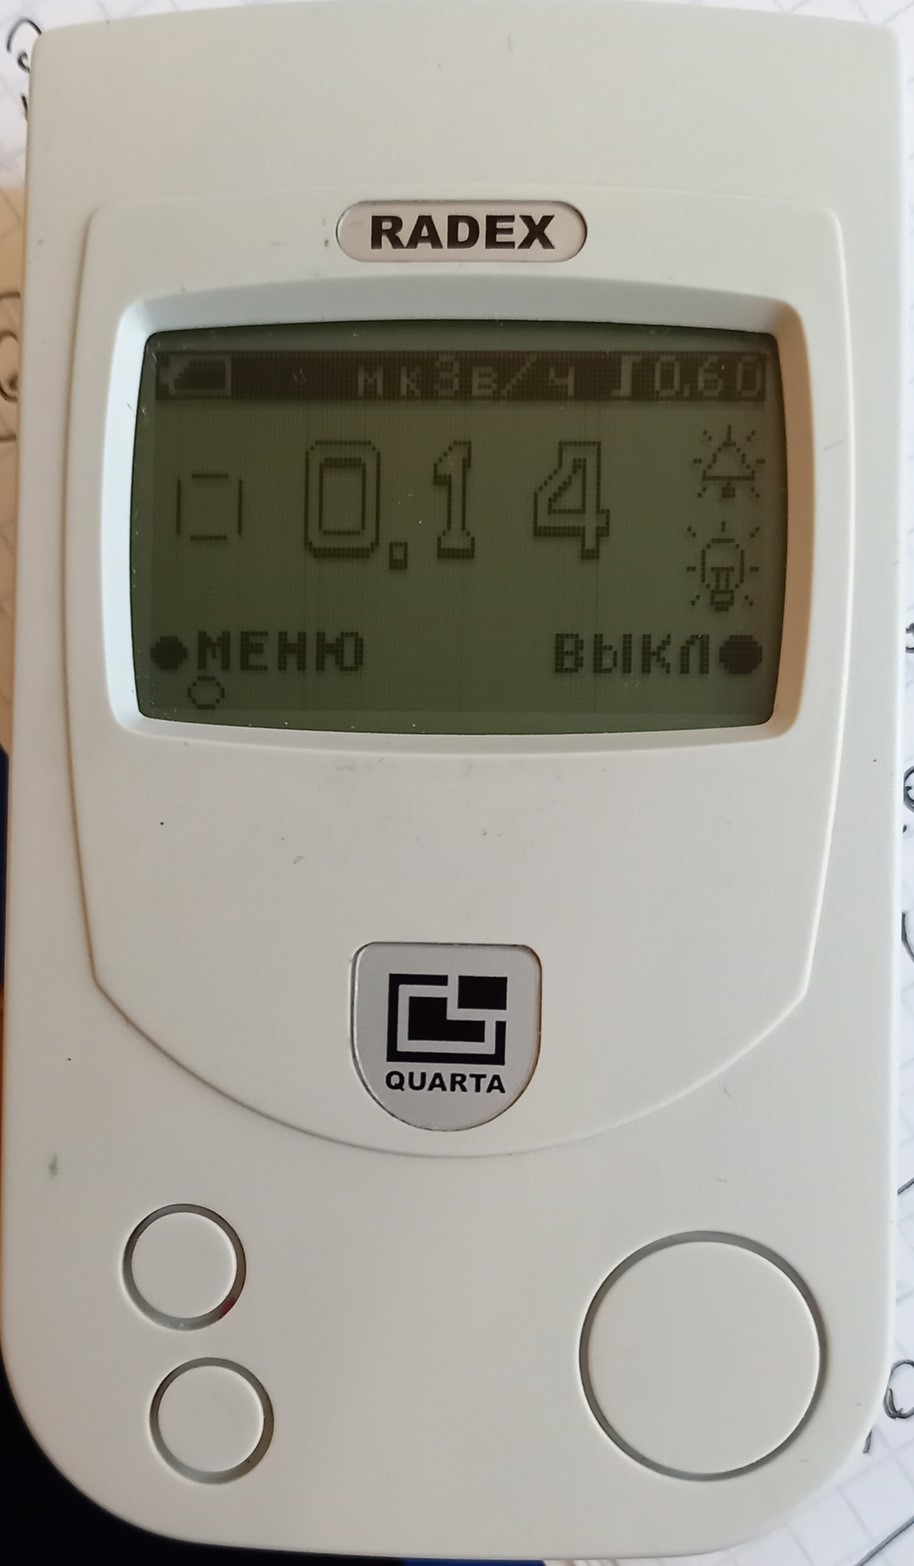
\includegraphics[scale=0.2]{fig3} 
	\caption{Дозиметр RADEX}
	\label{Radex}
\end{figure}

Измерим 	радиационный фон в нескольких местах лаборатории с помощью дозиметра Radex (представлен на рис \ref{Radex}).

Получили, что в комнате (вдали от источника) радиационный фон составляет 0,26 мкЗв/ч, а за 100 мм алюминия (при открытом источнике) -- 6,7 мкЗв/ч. 

Оценим вред здоровью человека: безопасная норма радиационного фона для человека -- 3-4 мЗв в год. Следовательно, чтобы получить годовую норму фона необходимо находится в комнате $\sim$ 1.3 года, а для 100 мм алюминия -- 20 часов.

\section*{Выводы}

\begin{itemize}
	\item В ходе лабораторной работы, были получены линейные коэффициенты поглощения $\gamma$-лучей для образцов из железа, алюминия и свинца.

\begin{table}[h]
	\centering
	\begin{tabular}{|c|c|}
	\hline
	\textbf{$\mu$, $см^{-1}$} & \textbf{Образец} \\ \hline
	1,13 $\pm$ 0,03 & свинец \\ \hline
	0,484 $\pm$ 0,005 & железо \\ \hline
	0,197 $\pm$ 0,001 & алюминий \\ \hline
\end{tabular}
\end{table}	

Данные значения коэффициента поглощения соответствуют энергиям $\gamma$-квантов, таким что $E_{\gamma} \in [0,6 \ МэВ ; 1,0 \ МэВ]$, значит энергия $\gamma$-квантов, испускаемых образцом, также лежит в данном диапазоне.

	\item Более того, были получены практические навыки работы с дозиметром, и было установлено, что никакого серьезного вреда здоровью лабораторные работы по общей физике не несут.
	
\end{itemize}

\newpage

\section*{Приложение}

\begin{table}[h]
	\caption{Измерения зависимости логарифма отношения потоков частиц от толщины образца для свинца}
	\label{table1}
	\centering
	\begin{tabular}{|c|c|c|}
	\hline
	\multicolumn{1}{|l|}{\textbf{l, см}} & \multicolumn{1}{l|}{\textbf{$\ln(N_0/N)$}} & \textbf{$\sigma_l$, см} \\ \hline
	0,5 & 0,636 & 0,100 \\ \hline
	1,01 & 1,230 & 0,141 \\ \hline
	1,5 & 1,784 & 0,173 \\ \hline
	2,02 & 2,167 & 0,200 \\ \hline
	2,46 & 2,748 & 0,224 \\ \hline
	\end{tabular}
\end{table}

\begin{table}[h]
	\caption{Измерения зависимости логарифма отношения потоков частиц от толщины образца для алюминия}
	\label{table2}
	\centering
	\begin{tabular}{|c|c|c|}
	\hline
	\multicolumn{1}{|l|}{\textbf{l, см}} & \multicolumn{1}{l|}{\textbf{$\ln(N_0/N)$}} & \textbf{$\sigma_l$, см} \\ \hline 
	2,1 & 0,427 & 0,100 \\ \hline
	4,07 & 0,821 & 0,141 \\ \hline
	6,17 & 1,219 & 0,173 \\ \hline
	8,15 & 1,622 & 0,200 \\ \hline
	10,25 & 1,985 & 0,223 \\ \hline
	\end{tabular}
\end{table}

\begin{table}[h]
	\caption{Измерения зависимости логарифма отношения потоков частиц от толщины образца для железа}
	\label{table3}
	\centering
	\begin{tabular}{|c|c|c|}
	\hline
	\multicolumn{1}{|l|}{\textbf{l, см}} & \multicolumn{1}{l|}{\textbf{$\ln(N_0/N)$}} & \textbf{$\sigma_l$, см} \\ \hline
	1,1 & 0,592 & 0,100 \\ \hline
	2,3 & 1,165 & 0,141 \\ \hline
	3,5 & 1,717 & 0,173 \\ \hline
	4,7 & 2,263 & 0,200 \\ \hline
	5,8 & 2,765 & 0,223 \\ \hline
	\end{tabular}
\end{table}


\end{document}
